\documentclass[xetex,mathserif,serif]{beamer}
\usepackage{polyglossia}
\setdefaultlanguage[babelshorthands=true]{russian}
\usepackage{minted}
\usepackage{tabu}
\usepackage[11pt]{moresize}

\usepackage{textpos}
\setlength{\TPHorizModule}{1cm}
\setlength{\TPVertModule}{1cm}

\useoutertheme{infolines}

\usepackage{fontspec}
\setmainfont{FreeSans}
\newfontfamily{\russianfonttt}{FreeSans}

\definecolor{links}{HTML}{2A1B81}
\hypersetup{colorlinks,urlcolor=links}
\hypersetup{linkcolor=}

\newcommand{\attribution}[1] {
	\vspace{-5mm}\begin{flushright}\begin{scriptsize}\textcolor{gray}{\textcopyright\, #1}\end{scriptsize}\end{flushright}
}

\tabulinesep=0.7mm

\title{Лекция 13: Проектирование распределённых приложений}
\subtitle{Часть первая: транспортные вопросы}
\author[Юрий Литвинов]{Юрий Литвинов \newline \textcolor{gray}{\small\texttt{yurii.litvinov@gmail.com}}}

\date{07.05.2019г}

\begin{document}
	
	\frame{\titlepage}

	\section{Введение}

	\begin{frame}
		\frametitle{Распределённые системы}
		\begin{itemize}
			\item Компоненты приложения находятся в компьютерной сети
			\item Взаимодействуют через обмен сообщениями
			\item Основное назначение --- работа с общими ресурсами
			\item Особенности
			\begin{itemize}
				\item Параллельная работа
				\item Независимые отказы
				\item Отсутствие единого времени
			\end{itemize}
		\end{itemize}
	\end{frame}

	\begin{frame}
		\frametitle{Частые заблуждения при проектировании распределённых систем}
		\begin{itemize}
			\item Сеть надёжна
			\item Задержка (latency) равна нулю
			\item Пропускная способность бесконечна
			\item Сеть безопасна
			\item Топология сети неизменна
			\item Администрирование сети централизовано
			\item Передача данных ``бесплатна''
			\item Сеть однородна
		\end{itemize}
	\end{frame}

	\section{Архитектура распределённых систем}

	\begin{frame}
		\frametitle{Архитектура распределённых систем}
		\begin{itemize}
			\item Какие сущности взаимодействуют между собой в распределённой системе?
			\item Как они взаимодействуют?
			\item Какие (возможно изменяющиеся) роли и ответственности имеют эти сущности в рамках всей архитектуры?
			\item Как они размещаются на физическую инфраструктуру?
		\end{itemize}
	\end{frame}

	\begin{frame}
		\frametitle{Виды сущностей}
		\begin{itemize}
			\item Узлы-процессы-потоки --- сущности уровня ОС (или сами вычислительные узлы, если ОС не поддерживает даже процессы)
			\item Объекты --- обычные объекты из ООП, с интерфейсами, описанными на IDL, вызыввающие друг друга по сети
			\item Компоненты --- более высокоуровневые сущности, как правило, предполагают middleware
			\item Веб-сервисы --- ещё более высокоуровневые сущности, независимые приложения с чётко определённым способом их использовать
		\end{itemize}
	\end{frame}

	\begin{frame}
		\frametitle{Виды взаимодействия}
		\begin{itemize}
			\item Межпроцессное взаимодействие
			\item Удалённые вызовы
			\begin{itemize}
				\item Протоколы вида ``запрос-ответ''
				\item Удалённые вызовы процедур (remote procedure calls, RPC)
				\item Удалённые вызовы методов (remote method invocation, RMI)
			\end{itemize}
			\item Неявное взаимодействие
			\begin{itemize}
				\item Групповое взаимодействие
				\item Модель “издатель-подписчик”
				\item Очереди сообщений
				\item Распределённая общая память
			\end{itemize}
		\end{itemize}
	\end{frame}

	\begin{frame}
		\frametitle{Роли и обязанности}
		\begin{itemize}
			\item Клиент-сервер
			\item Peer-to-peer
		\end{itemize}
	\end{frame}

	\begin{frame}
		\frametitle{Варианты размещения}
		\begin{itemize}
			\item Разбиение сервисов по нескольким серверам
			\item Кэширование
			\item Мобильный код
			\item Мобильный агент
		\end{itemize}
	\end{frame}

	\begin{frame}
		\frametitle{Типичные архитектурные стили}
		\begin{itemize}
			\item Уровневая архитектура
			\begin{itemize}
				\item ОС
				\item Коммуникационная инфраструктура (Middleware)
				\item Приложения и сервисы
			\end{itemize}
			\item Клиент-сервер
			\begin{itemize}
				\item Тонкий клиент
				\item Бизнес-логика и данные --- на сервере
			\end{itemize}
			\item Трёхзвенная и N-уровневая архитектуры
			\begin{itemize}
				\item Бизнес-логику и работу с данными часто разделяют
			\end{itemize}
		\end{itemize}
	\end{frame}

	\section{Сетевое взаимодействие}

	\begin{frame}
		\frametitle{Модель OSI}
		\begin{center}
			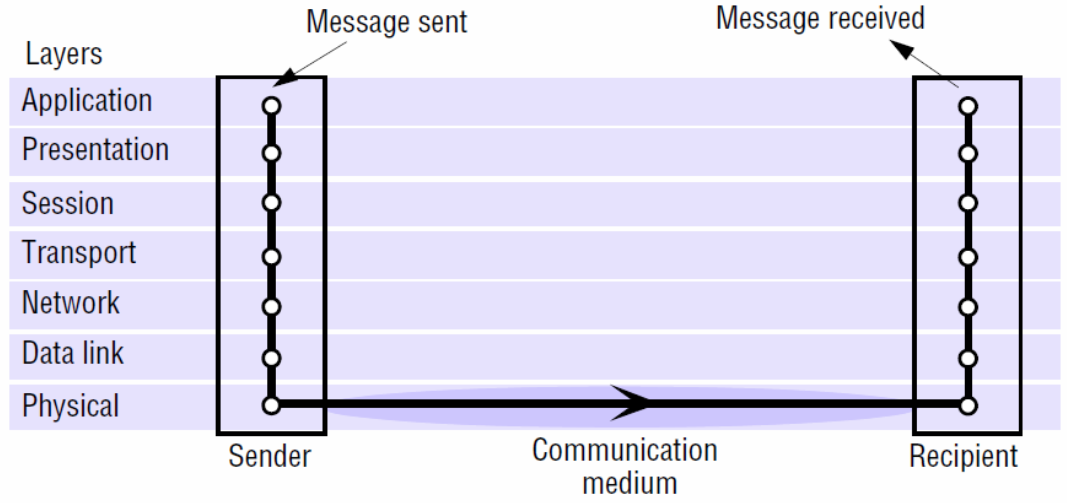
\includegraphics[width=0.8\textwidth]{osiStack.png}
		\end{center}
	\end{frame}

	\begin{frame}
		\frametitle{Стек протоколов TCP/IP}
		\begin{center}
			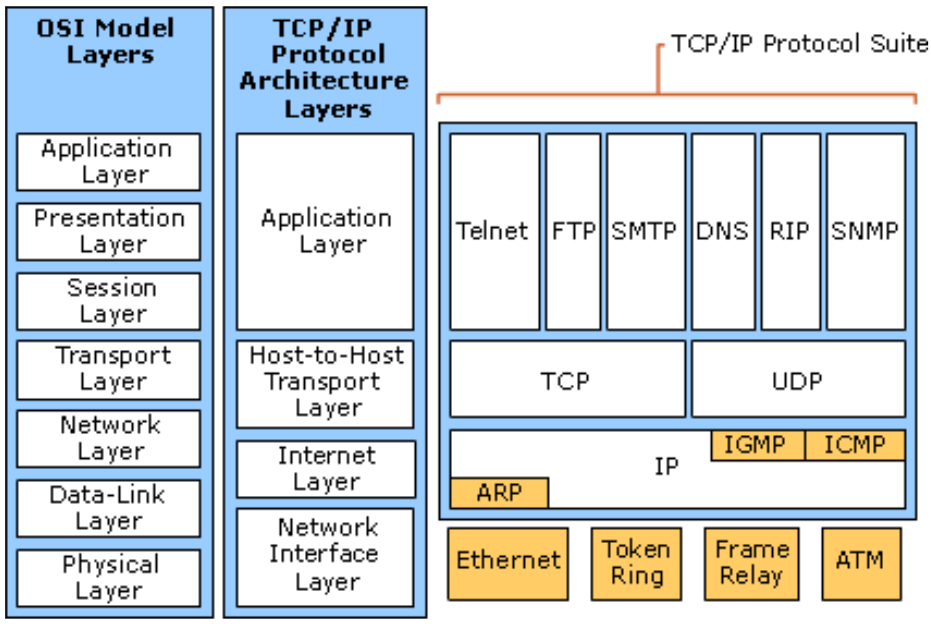
\includegraphics[width=0.8\textwidth]{tcpIpStack.png}
		\end{center}
	\end{frame}

	\begin{frame}
		\frametitle{Абстракция сокета}
		\begin{center}
			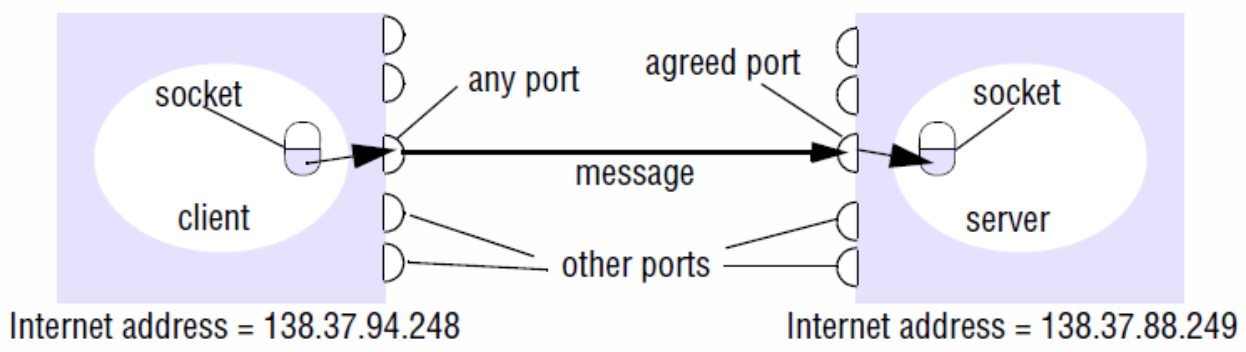
\includegraphics[width=0.8\textwidth]{sockets.png}
		\end{center}
	\end{frame}

	\section{Протоколы ``запрос-ответ''}

	\begin{frame}
		\frametitle{Протоколы ``запрос-ответ''}
		\begin{itemize}
			\item Запрос, действие, ответ
			\item Преимущественно синхронные вызовы
		\end{itemize}
		\begin{center}
			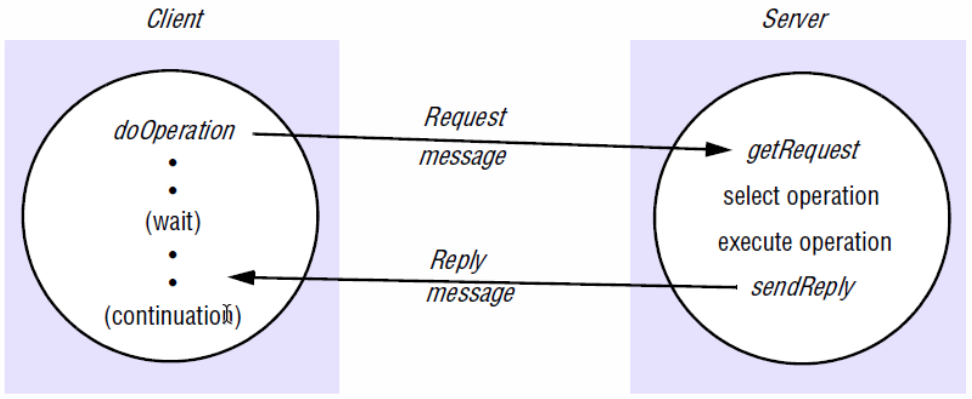
\includegraphics[width=0.8\textwidth]{requestReplyProtocols.png}
		\end{center}
	\end{frame}

	\begin{frame}
		\frametitle{``Запрос-ответ'' поверх UDP}
		\begin{itemize}
			\item[+] Уведомления не нужны
			\item[+] Установление соединения --- в два раза больше сообщений
			\item[+] Управление потоком не имеет смысла
			\item[-] Потери пакетов
			\begin{itemize}
				\item Таймаут + повторный запрос на уровне бизнес-логики
				\item Защита от повторного выполнения операции (хранение ``истории'')
				\item Новый запрос как подтверждение получения прошлого
			\end{itemize}
			\item[-] Неопределённый порядок пакетов
		\end{itemize}
	\end{frame}

	\begin{frame}
		\frametitle{``Запрос-ответ'' поверх TCP}
		\begin{itemize}
			\item[+] Использование потоков вместо набора пакетов
			\begin{itemize}
				\item Удобная отправка больших объёмов данных
				\item Один поток на всё взаимодействие
			\end{itemize}
			\item[+] Интеграция с потоками ОО-языков
			\item[+] Надёжность доставки
			\begin{itemize}
				\item Отсутствие необходимости проверок на уровне бизнес-логики
				\item Уведомления в пакетах с ответом
				\item Упрощение реализации
			\end{itemize}
			\item[-] Тяжеловесность коммуникации
		\end{itemize}
	\end{frame}

	\section{HTTP}

	\begin{frame}
		\frametitle{HTTP}
		\begin{itemize}
			\item Пример протокола ``запрос-ответ''
			\item Реализован поверх TCP
			\item Соединение на всё время взаимодействия
			\item Маршалинг данных в ASCII
			\begin{itemize}
				\item MIME
			\end{itemize}
			\item HTTP 2.0
			\begin{itemize}
				\item Бинарный протокол
				\item Обязательное шифрование
				\item Мультиплексирование запросов в одном TCP соединении
				\item ``Предсказывающая посылка данных''
			\end{itemize}
		\end{itemize}
	\end{frame}

	\section{RPC}

	\begin{frame}
		\frametitle{RPC}
		\begin{center}
			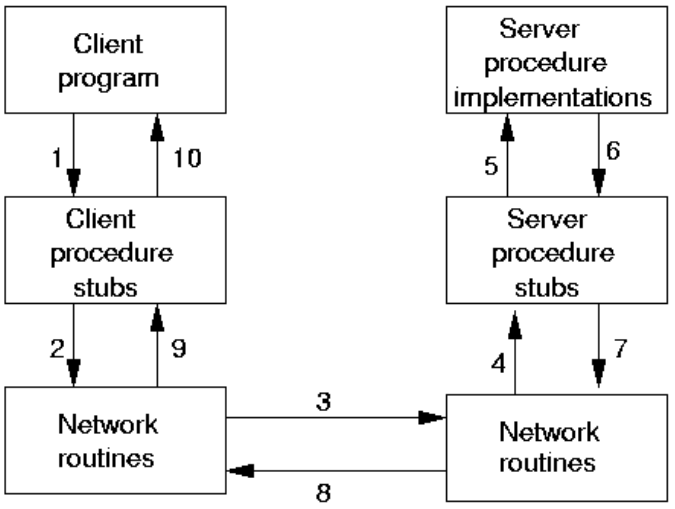
\includegraphics[width=0.6\textwidth]{rpc.png}
		\end{center}
	\end{frame}

	\begin{frame}
		\frametitle{Прозрачность RPC-вызовов}
		\begin{itemize}
			\item Изначальная цель --- максимальная похожесть на обычные вызовы
			\begin{itemize}
				\item Location and access transparency
			\end{itemize}
			\item Удалённые вызовы более уязвимы к отказам
			\begin{itemize}
				\item Нужно понимать разницу между отказом сети и отказом сервиса
				\begin{itemize}
					\item Exponential backoff
				\end{itemize}
				\item Клиенты должны знать о задержках при передаче данных
				\begin{itemize}
					\item Возможность прервать вызов
				\end{itemize}
			\end{itemize}
			\item Явная маркировка удалённых вызовов?
			\begin{itemize}
				\item Прозрачность синтаксиса
				\item Явное отличие в интерфейсах
				\begin{itemize}
					\item Указание сематики вызова
				\end{itemize}
			\end{itemize}
		\end{itemize}
	\end{frame}

	\begin{frame}
		\frametitle{Структура RPC middleware}
		\begin{center}
			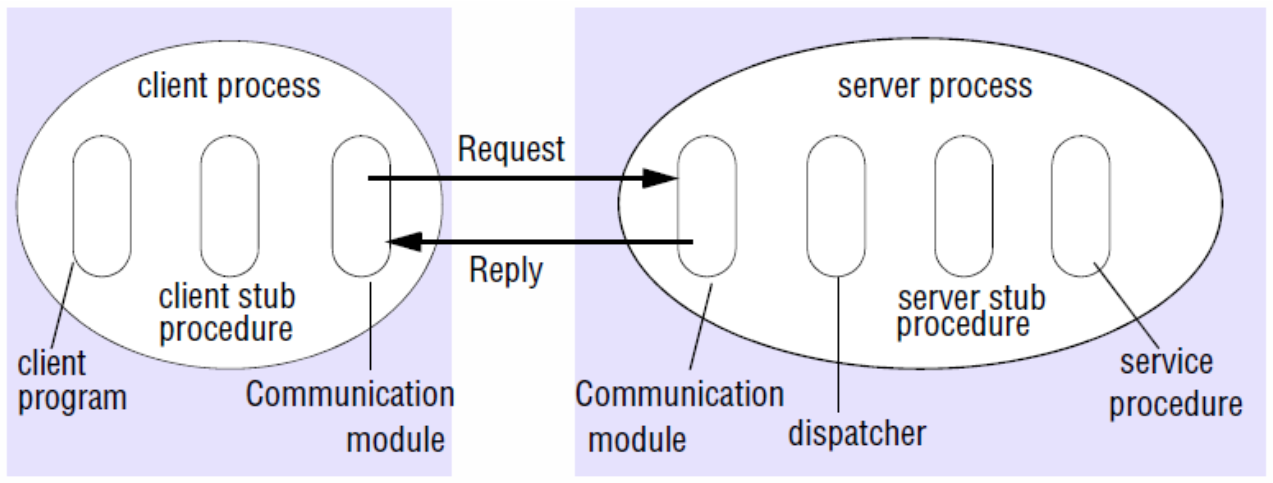
\includegraphics[width=0.8\textwidth]{rpcMiddlewareArchitecture.png}
		\end{center}
	\end{frame}

	\section{RMI}

	\begin{frame}
		\frametitle{Удалённые вызовы методов (RMI)}
		\begin{itemize}
			\item Продолжение идей RPC
			\begin{itemize}
				\item Программирование через интерфейсы
				\item Работа поверх протоколов ``запрос-ответ''
				\item At-least-once или at-most-once семантика вызовов
				\item Прозрачность синтаксиса вызовов
			\end{itemize}
			\item Особенности ОО-программ
			\begin{itemize}
				\item Наследование, полиморфизм
				\item Передача параметров по ссылкам
				\item Исключения
				\item Распределённая сборка мусора
			\end{itemize}
		\end{itemize}
	\end{frame}

	\begin{frame}
		\frametitle{Локальные и удалённые вызовы}
		\begin{itemize}
			\item Локальные и удалённые объекты
			\item Интерфейсы удалённых объектов
			\item Ссылки на удалённые объекты
			\begin{itemize}
				\item Как параметры или результаты удалённых вызовов
			\end{itemize}
		\end{itemize}
		\begin{center}
			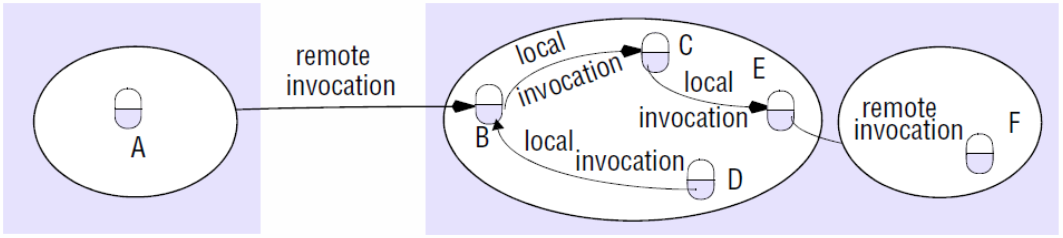
\includegraphics[width=0.8\textwidth]{remoteCalls.png}
		\end{center}
	\end{frame}

	\begin{frame}
		\frametitle{Структура RMI middleware}
		\begin{center}
			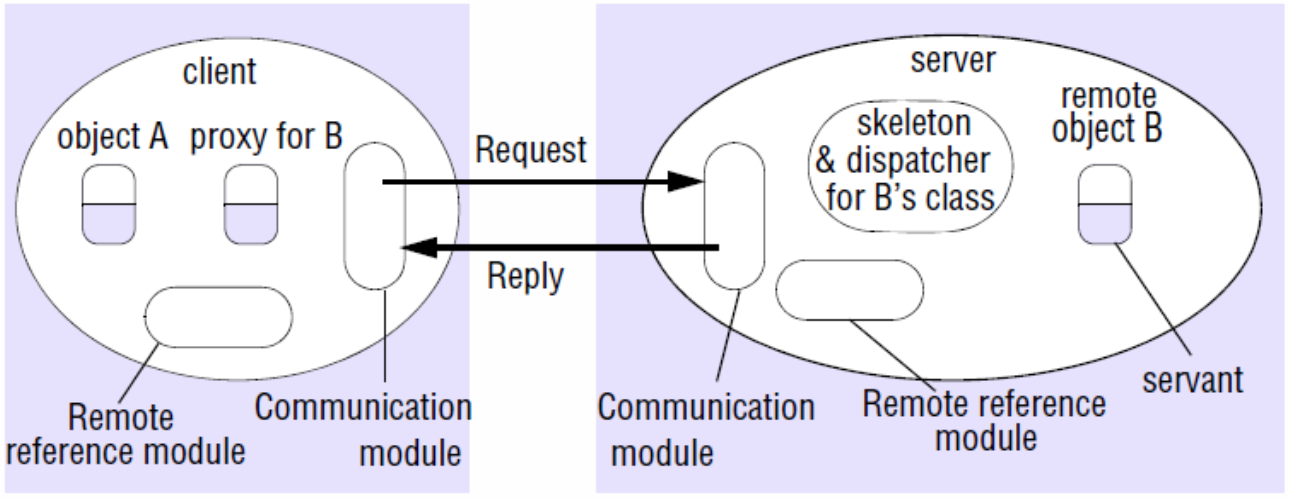
\includegraphics[width=0.8\textwidth]{rmiArchitecture.png}
		\end{center}
	\end{frame}

	\section{protobuf}

	\begin{frame}
		\frametitle{Protocol buffers}
		\framesubtitle{protobuf}
		\begin{itemize}
			\item Механизм сериализации-десериализации данных
			\item Компактное бинарное представление
			\item Декларативное описание формата данных, генерация кода для языка программирования
			\begin{itemize}
				\item Поддерживается Java, Python, Objective-C, C++, Go, JavaNano, Ruby, C\#
			\end{itemize}
			\item Бывает v2 и v3, с некоторыми синтаксическими отличиями
			\item Хитрый протокол передачи, \url{https://developers.google.com/protocol-buffers/docs/encoding}
			\begin{itemize}
				\item До 10 раз компактнее XML 
			\end{itemize}
		\end{itemize}
	\end{frame}

	\begin{frame}[fragile]
		\frametitle{Пример}
		Файл .proto:
		\begin{minted}{protobuf}
message Person {
  required string name = 1;
  required int32 id = 2;
  optional string email = 3;
}
		\end{minted}
		\vspace{2mm}
		Файл .java:
		\begin{minted}{java}
Person john = Person.newBuilder()
    .setId(1234)
    .setName("John Doe")
    .setEmail("jdoe@example.com")
    .build();
output = new FileOutputStream(args[0]);
john.writeTo(output);
		\end{minted}
	\end{frame}

	\section{gRPC}

	\begin{frame}
		\frametitle{gRPC}
		\begin{columns}
			\begin{column}{0.6\textwidth}
				\begin{itemize}
					\item средство для удалённого вызова (RPC)
					\item Работает поверх protobuf
					\item Разрабатывается Google
					\item Поддерживает C++, Java, Objective-C, Python, Ruby, Go, C\#, Node.js
				\end{itemize}
			\end{column}
			\begin{column}{0.4\textwidth}
				\begin{center}
					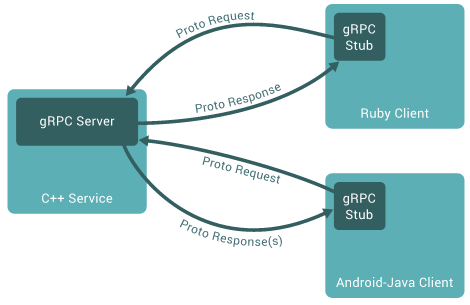
\includegraphics[width=\textwidth]{grpc.png}
				\end{center}
			\end{column}
		\end{columns}
	\end{frame}

	\begin{frame}[fragile]
		\frametitle{Технические подробности}
		\begin{itemize}
			\item Сервисы описываются в том же .proto-файле, что и протокол protobuf-а
			\item В качестве типов параметров и результатов --- message-и protobuf-а
		\end{itemize}
		\begin{minted}{protobuf}
service RouteGuide {
  rpc GetFeature(Point) returns (Feature) {}
  rpc ListFeatures(Rectangle) returns (stream Feature) {}
  rpc RecordRoute(stream Point) returns (RouteSummary) {}
  rpc RouteChat(stream RouteNote) returns (stream RouteNote) {}
}
		\end{minted}
		\begin{itemize}
			\item Сборка --- плагином grpc к protoc
		\end{itemize}
\end{frame}

	\begin{frame}[fragile]
		\frametitle{Реализация сервиса на Java}
		\begin{scriptsize}
			\begin{minted}{java}
private static class RouteGuideService extends RouteGuideGrpc.RouteGuideImplBase {
    ...
    @Override
    public void getFeature(Point request, StreamObserver<Feature> responseObserver) {
      responseObserver.onNext(checkFeature(request));
      responseObserver.onCompleted();
    }

    @Override
    public void listFeatures(Rectangle request, StreamObserver<Feature> responseObserver) {
      for (Feature feature : features) {
        ...
        int lat = feature.getLocation().getLatitude();
        int lon = feature.getLocation().getLongitude();
        if (lon >= left && lon <= right && lat >= bottom && lat <= top) {
          responseObserver.onNext(feature);
        }
      }
      responseObserver.onCompleted();
    }
			\end{minted}
		\end{scriptsize}
	\end{frame}

	\begin{frame}[fragile]
		\frametitle{Реализация сервиса на Java (2)}
		\begin{scriptsize}
			\begin{minted}{java}
    @Override
    public StreamObserver<RouteNote> routeChat(
            final StreamObserver<RouteNote> responseObserver) {
      return new StreamObserver<RouteNote>() {
        @Override
        public void onNext(RouteNote note) {
          List<RouteNote> notes = getOrCreateNotes(note.getLocation());
          for (RouteNote prevNote : notes.toArray(new RouteNote[0])) {
            responseObserver.onNext(prevNote);
          }
          notes.add(note);
        }
        @Override
        public void onError(Throwable t) {
          logger.log(Level.WARNING, "routeChat cancelled");
        }
        @Override
        public void onCompleted() {
          responseObserver.onCompleted();
        }
      };
    }
			\end{minted}
		\end{scriptsize}
	\end{frame}

	\begin{frame}[fragile]
		\frametitle{Реализация клиента на Java (1)}
		\begin{scriptsize}
			\begin{minted}{java}
public RouteGuideClient(String host, int port) {
    this(ManagedChannelBuilder.forAddress(host, port).usePlaintext(true));
}

public RouteGuideClient(ManagedChannelBuilder<?> channelBuilder) {
    channel = channelBuilder.build();
    blockingStub = RouteGuideGrpc.newBlockingStub(channel);
    asyncStub = RouteGuideGrpc.newStub(channel);
}
			\end{minted}
		\end{scriptsize}
	\end{frame}

	\begin{frame}[fragile]
		\frametitle{Реализация клиента на Java (2)}
		\begin{scriptsize}
			\begin{minted}{java}
public void getFeature(int lat, int lon) {
    Point request = Point.newBuilder().setLatitude(lat).setLongitude(lon).build();
    Feature feature;
    try {
        feature = blockingStub.getFeature(request);
    } catch (StatusRuntimeException e) {
        warning("RPC failed: {0}", e.getStatus());
        return;
    }
    if (RouteGuideUtil.exists(feature)) {
        info("Found feature called \"{0}\" at {1}, {2}",
            feature.getName(),
            RouteGuideUtil.getLatitude(feature.getLocation()),
            RouteGuideUtil.getLongitude(feature.getLocation()));
    } else {
        info("Found no feature at {0}, {1}",
            RouteGuideUtil.getLatitude(feature.getLocation()),
            RouteGuideUtil.getLongitude(feature.getLocation()));
    }
}
			\end{minted}
		\end{scriptsize}
	\end{frame}

	\section{Веб-сервисы}

	\begin{frame}
		\frametitle{Веб-сервисы}
		\begin{itemize}
			\item Перенос специализации клиент-сервера в web
			\item Cложные приложения как интеграция веб-сервисов
			\item HTTP-запрос для выполнения команды
			\begin{itemize}
				\item Aсинхронное взаимодействие
				\item Ответ-запрос
				\item Событийные схемы
			\end{itemize}
			\item XML или JSON как основной формат сообщений
			\begin{itemize}
				\item SOAP/WSDL/UDDI
				\item XML-RPC
				\item REST
			\end{itemize}
		\end{itemize}
	\end{frame}

\end{document}
